\documentclass{report}

\usepackage{float}
\usepackage{url}
\usepackage{graphicx}
\usepackage{listings}
\usepackage{color}
\usepackage{verbatim}
\usepackage[lined,linesnumbered,algochapter]{algorithm2e}
\usepackage{tikz}
\usetikzlibrary{arrows,automata}
\usepackage{xspace}
\usepackage{caption}
%\usepackage[colorlinks = true, urlcolor  = blue]{hyperref}
\usepackage{ucs}
\usepackage[utf8]{inputenc}

%\hypersetup{colorlinks=false, linkcolor=red}

\usepackage{ngerman}
\usepackage[ngerman, english]{babel}
\usepackage{bibgerm,cite}       % Deutsche Bezeichnungen, Automatisches Zusammenfassen von Literaturstellen
\usepackage[ngerman]{varioref}  % Querverweise

\DeclareCaptionFont{white}{\color{white}}
\DeclareCaptionFormat{listing}{\colorbox{gray}{\parbox{\textwidth}{#1#2#3}}}
\captionsetup[lstlisting]{format=listing,labelfont=white,textfont=white}

\lstset{language=Java,captionpos=b,tabsize=3,frame=lines,keywordstyle=\color{blue},commentstyle=\color{darkgreen},stringstyle=\color{red},numbers=left,numberstyle=\tiny,numbersep=5pt,breaklines=true,showstringspaces=false,basicstyle=\footnotesize,emph={label}}

\setcounter{secnumdepth}{2}
\setcounter{tocdepth}{3}

% another code presentation stlye
%\definecolor{dkgreen}{rgb}{0,0.6,0}
%\definecolor{gray}{rgb}{0.5,0.5,0.5}
%\definecolor{mauve}{rgb}{0.58,0,0.82}
%
%\lstset{frame=tb,
%  language=Java,
%  aboveskip=3mm,
%  belowskip=3mm,
%  showstringspaces=false,
%  columns=flexible,
%  basicstyle={\small\ttfamily},
%  numbers=none,
%  numberstyle=\tiny\color{gray},
%  keywordstyle=\color{blue},
%  commentstyle=\color{dkgreen},
%  stringstyle=\color{mauve},
%  breaklines=true,
%  breakatwhitespace=true
%  tabsize=3
%}

% define custom macros for specific formats or names
\newcommand{\uml}[1]{\texttt{#1}}
\newcommand{\cd}{\textsf{Class Diagram}}

\begin{document}
\pagestyle{plain}
\pagenumbering{roman}

\title{Risikomanagement}


\maketitle

\tableofcontents
\newpage

\pagenumbering{arabic}

% Kapitel
% --------------------------------------------------------------
\chapter{Definition und Grundlagen Risikomanagement}
\label{sect:grundlagen}


% --------------------------------------------------------------
\chapter{Software, Plattformen und Apps im Risikomanagement}

\section{Einleitung}

In den letzten Jahren wurde viel in die Entwicklung von Systemen die Risiko messbar machen investiert. Risikomessung ist stets eine passive Aktivität. Risikomanagement ist ein dynamisches bestreben und benötigt Tools und Anwendungen die beim identifizieren und verringern der Risikoquellen helfen. \cite{Mausser1997} 
NASA ist wegweisend in diesem Bereich. Die Steuerung von Risiko wird als Resource angesehen die gehandelt werden kann gegen andere Resourcen wie Zeit, Kosten oder Leistung. Ein erfolgreiches Risikomanagement beinhaltet also das Identifizieren des Risikos, das Abschätzen der Auswirkungen und der Eintrittswahrscheinlichkeit, das Entscheiden welche Risiko-level akzeptabel sind und die Risikominimierung.\cite{Feather2000}

In den Anfangsphasen eines Projektes ist Risikomanagement hauptsächlich qualitativ. Basierend auf den vorhandenen Informationen sind die Risiken kategorisiert und normalerweise high-level. In späteren Phasen geht es mehr um Teilsysteme, Detailanforderungen und Herstellungs / Softwaremodelle. Risikomanagement ist jetzt primär quantitativ und nicht qualitativ. Die identifizierten Risiken sind sehr detailliert und fokussiert auf spezifische Probleme.\cite{Feather2000}


\section{Kategorien}

Um eine ordentliche Analyse durchzuführen ist es wichtig die Vorteile und Nachteile von Quantitativen und Qualitativen Risiken zu beachten.\cite{Stoneburner2002}

\subsection{Qualitativ}
Der groeste Vorteil von qualitativer Risikoanalyse ist das die Risiken priorisiert werden und bereits mögliche Verbesserungen in Betracht gezogen werden.
Mit der qualitativen Analyse ist is dafür schwierig abzuschätzen welche Kostenvorteile gewisse Gegenmaßnahmen haben, da keine messbaren Werte fuer das Ausmass der Risiken vorhanden sind.\cite{Stoneburner2002}
\subsection{Quantitativ}
Der Vorteil von quantitativer Risikoanalyse ist das es die Messbarkeit fuer das Ausmass von Risiken verbessert. Dadurch können die Kostenvorteile von Gegenmaßnahmen besser analysiert werden.
Im Gegensatz zur qualitativen Analyse ist das interpretieren der quantitativen Analyse schwieriger. Abhängig von den gemessenen Werten kann es sein das weitere Faktoren in Betracht gezogen werden muessen um die Ergebnisse zu verstehen.\cite{Stoneburner2002}

\subsection{Kombiniere Qualitativ und Quantitativ}
Sowohl die Qualitative als auch Quantitative Methode haben ihr Vorteile und Nachteile. Um auf ein gutes Ergebnis der Risikoanalyse zu kommen können beide kombiniert werden. Dadurch werden die Informationen im Gesamtbild betrachtet und eine Interpretation der Daten wird vereinfacht. Als Beispiel gilt hier das von der NASA verwendete Risk Balancing Profile fuer qualitative Daten und Defect Detection and Prevention fuer quantitative Daten. In \cite{Feather2000} werden diese beiden Tools vorgestellt und dargelegt wie eine Kombination daraus aussieht.

\section{Tools}
\subsection{Appthority}

\subsubsection{Beschreibung}
Appthority wurde 2011 gegründet mit einem einzigen Ziel, Firmen vor Sicherheits-, Datenverlust- und Privatsphäre Risiken zu schützen die durch schnell wachsende Mitarbeiterzahlen und die daraus resultierende Verwendung von mobilen Anwendungen entsteht. Es bietet eine einfache und skalierbare Möglichkeit diese Risiken zu beherrschen.\cite{AppthorityBlog}\cite{Appthority}

\begin{enumerate}
\item Die Appthority Datenbank beinhaltet mehr als 3 Millionen Anwendungen.
\item Vorerst nur iOS und Android unterstützt.
\item Blackberry 10 und Windows Phone apps sollen folgen.
\item Über 1 Millionen API Anfragen pro Tag
\end{enumerate}

\subsubsection{Anwendung}
Bis 2013 gab es bei Appthority nur die Möglichkeit über eine API die analysierten Daten zu erhalten. Seit 2 Jahren gibt es nun ein Webportal das ebenfalls dafür genutzt werden kann. An dieser zentralen Stelle kann fuer alle mobilen Geräte die von den Mitarbeitern einer Firma im Umlauf sind eine Riskoanalyse durchgeführt werden. Dabei werden sämtliche sich auf den Geräten befindenden Anwendungen mit der jeweiligen Versionsnummer von Appthority kontrolliert. Befinden sich potentiell gefährliche Anwendungen auf einem Gerät, werden die zuständigen IT Fachkräfte darüber informiert. \ref{fig:appthority} \cite{AppthorityBlog}\cite{Appthority}

\subsubsection{Appthorities Analyse}
\begin{enumerate}
\item Statische und dynamische Analyse des Binaerfiles 
\item Über 3000 Regeln die kontrolliert werden
\item Wie verhält sich die Anwendung?
\item Aus welchem Land kommt die Anwendung?
\item Von welchen Entwicklern wurde die Anwendung entwickelt?
\item Welchen anderen Referenzen haben diese Entwickler?
\end{enumerate}

\begin{figure}[h!]
  \centering
  \fbox{
    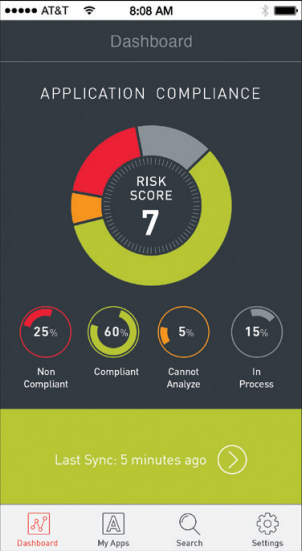
\includegraphics[width=0.4 \textwidth]{./Images/appthority.png}
  }
  \caption{Appthority}
  \label{fig:appthority}
\end{figure}

\subsection{IntelliRisk}
\subsubsection{Beschreibung}

IntelliRisk ist ein Produkt der American International Group, einer der international führenden Versicherungsorganisation tätig in über 130 Ländern. Es bietet schnellen und einfachen Zugang zu Informationen und die Möglichkeit Reports zu erstellen. AIG bietet auch eine erweiterte Variante mit dem Namen IntelliRisk Advanced an. Diese verfügt über komplexere Risiko und Forderungsfeatures.\cite{AIG}
\begin{enumerate}
\item interaktives Dashboard
\item real-time Zugriff auf Aktivitätsnotizen
\item Alarmsystem bei signifikanten Veraenderungen
\item konfigurierbare Reports
\item Identifikation von hohen Kosten
\item mobile Version
\end{enumerate}


\subsection{SaS for Enterprise Risk Management}
\subsubsection{Beschreibung}
SAS bietet durchgängige Softwarelösungen für den gesamten Prozess des Risikomanagements. Angefangen von der Datenaufbereitung bis über Risikokalkulation, Aggregation und Reporting. Egal ob Finanzkennzahlen, Produkt- und Kundendaten, Marktinformationen oder operative Messgrößen, mit SAS werden die enormen Datenmengen aus allen operativen Systemen integriert und für die Risikosteuerung nutzbar. Korrelationen zwischen Risikoarten werden sichtbar und verbessern den Umgang damit.

\begin{enumerate}
\item Nachweis der ordnungsgemäßen Umsetzung der GRC-Regularien.
\item Echtzeit Dashboard
\item Alarmsystem
\end{enumerate}

\subsection{IntelligenceBank GRC}

\subsubsection{Beschreibung}
IntelligenceBank GRC ist eine Platform as a Service Lösung aus Australien. Risikomanager können innerhalb dieser Platform Risiken, Vorfälle und andere firmen interne Daten eintragen. Diese analysierten und aufgeschlüsselten Daten können dem Firmenmanagement und Stakeholdern präsentiert werden, die somit jederzeit einen klaren Überblick über aktuelle Risiken und deren Status haben.
\subsubsection{Anwendung}
In der Webanwendung ist die Register-Ansicht eine der wichtigsten. Die bereits vorhandenen wie Risiko, Gesundheit, Vertrag, Unfälle oder Kunden können nach belieben erweitert werden um den jeweiligen Anforderungen zu entsprechen. Zu jedem dieser Register gehört ein bestimmter Eingabeprozess der angepasst werden kann.\cite{intelligencebank}

\subsection{Citicus MOCA}
\subsubsection{Beschreibung}
Im Unterschied zu den bis jetzt angeführten Lösungen ist Citicus MOCA eine reine iPhone Anwendung. Die App laesst den Benutzer alle möglichen beeinflussenden Faktoren eintragen und diese bewerten, um anschliessend ein Ergebnis daraus zu ziehen.\cite{Citicus}

\begin{enumerate}
\item Informationssysteme
\item IT Infrastruktur (Datencenter)
\item IT Service Anbieter
\item Fabriken
\item Bueros
\item ...
\end{enumerate}

\subsubsection{Anwendung}

Zuerst werden sämtliche Firmen relevanten Ressourcen in der App eingetragen. Diese werden dann von verschiedenen Perspektiven betrachtet und Risiken werden identifiziert. Anhand einer vorgegebenen Skala wird dann jedes Risiko bewertet \ref{fig:citicus}. Der maximal mögliche Verlust wird zum Schluss über einen übersichtlich gestalteten Report angezeigt. Der Prozess funktioniert sehr schnell wodurch sich die App hervorragend fuer eine schnelle Entscheidungshilfe unterwegs eignet.\cite{Citicus}

\begin{figure}[h!]
  \centering
  \fbox{
    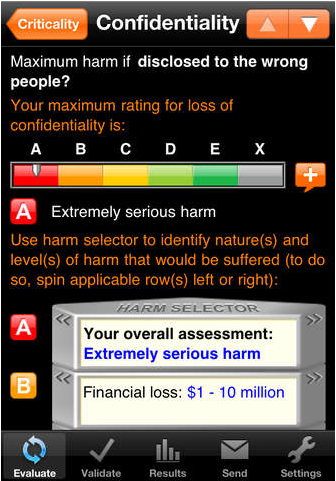
\includegraphics[width=0.4 \textwidth]{./Images/Citicus_MOCA_1.png}
  }
  \caption{Citicus}
  \label{fig:citicus}
\end{figure}

\section{Zusammenfassung}

Im Enterprise Bereich existieren eine Vielzahl an Softwarelösungen fuer Risikomanagement. Die meisten davon sind sehr breit aufgestellt und versuchen möglichst viele Anwendungsfaelle abzudecken. Dadurch sind sie auch eher fuer mittelgrosse bis grosse Firmen geeignet.
Neben diesem Enterprisemarkt gibt es auch einen Markt fuer Teilproblemlösungen. Dafür eignen sich auch durchaus mobile Anwendungen die auf Android oder iOS laufen.


















% --------------------------------------------------------------
\chapter{Risikomanagement im Bereich Service und Data Clouds}
\label{sect:clouds}



% --------------------------------------------------------------
\chapter{Risikomanagnement im Kontext von Smart Technologien}
\label{sect:relevance}


\bibliographystyle{acm}
\bibliography{risk2015}

\end{document}
